%%%%%%%%% PROJECT DESCRIPTION  -- 15 pages (including Prior NSF Support)

\required{Project Description}
\begin{center}
%\emph{Maximum of 15 pages}
\end{center}•
%The Project Description (including Results from Prior NSF Support, which is
%limited to five pages) may not exceed 15 pages. Visual materials, including charts,
%graphs, maps, photographs and other pictorial presentations are included in the
%15-page limitation. PIs be cautioned that the project description must
%be self-contained and that URLs that provide information related to the proposal
%should not be used. \\
%
%All proposals to NSF are reviewed utilizing the two merit review criteria,
%intellectual merit and broader impacts. \\
%
% The Project Description should provide a clear statement of the work 
% to be undertaken and must include: objectives for the period of the proposed 
% work and expected significance; relation to longer-term goals of the PI's 
% project; and relation to the present state of knowledge in the field, 
% to work in progress by the PI under other support and to work in progress 
% elsewhere.

%%%%%%%%%%%%%%%%%%%%%%%%%%%%%%%%%%%%%%%%%%%%%%%%%%%%%%%%%%%%%%%%%%%%%%
%INTRO
%%%%%%%%%%%%%%%%%%%%%%%%%%%%%%%%%%%%%%%%%%%%%%%%%%%%%%%%%%%%%%%%%%%%%%
\section*{Introduction}

why adaptation is important

%%%%%%%%%%%%%%%%%%%%%%%%%%%%%%%%%%%%%%%%%%%%%%%%%%%%%%%%%%%%%%%%%%%%%%
%AIMS
%%%%%%%%%%%%%%%%%%%%%%%%%%%%%%%%%%%%%%%%%%%%%%%%%%%%%%%%%%%%%%%%%%%%%%
\section*{Aims}

To investigate the genetics of adaptation in maize, we focus here on adaptation to high elevation. Maize has adapted to high elevations multiple times throughout its history, thus allowing us independently replicated natural experiments from which to sample the genetics of adaptation. Our project has three main aims:

\begin{enumerate}
\item {\bf Genetic architecture of highland traits}
\item {\bf Population genetics of maize-teosinte introgression}
\item {\bf Functional characterization of adaptive quantitative trait loci}
\end{enumerate}

%%%%%%%%%%%%%%%%%%%%%%%%%%%%%%%%%%%%%%%%%%%%%%%%%%%%%%%%%%%%%%%%%%%%%%
%RAIONALE AND SIGNIFICANCE
%%%%%%%%%%%%%%%%%%%%%%%%%%%%%%%%%%%%%%%%%%%%%%%%%%%%%%%%%%%%%%%%%%%%%%
\section*{Rationale and Significance}

\paragraph*{Maize is highly adaptive}

\begin{SCfigure}
  \centering
  \caption{Geographic breadth of the world's 16 most important crops. Geographic breadth is expressed in percent of land surface area in which each crop is cultiavated. Data from \citet{Ramankutty2008}. } 
   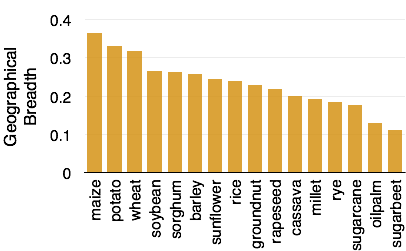
\includegraphics[width=0.6\textwidth]{breadth.png}

\label{fig:breadth}
\end{SCfigure}


\paragraph*{Maize adaptation is important for food security}

important for foods

population expansion -- need to grow more food in new places

climate change -- climate will change in places maize is grown

\paragraph*{We know almost nothing about genetics adaptation in maize}

we know lots about quant. traits in maize (temperate), but almost nothign about adaptive traits

genetic arch. can differ. e.g. time to flowering in temp maize lots of genes small effect, but diff. between trop and temp is few photoperiod loci of large effect -- so adaptation to temperate was predominantly a few loci of large effect even though the genetic arch. of flowering time among temperate is lots of loci of small effect (reference fisher?) cite brown et al. 2011

%%%%%%%%%%%%%%%%%%%%%%%%%%%%%%%%%%%%%%%%%%%%%%%%%%%%%%%%%%%%%%%%%%%%%%
%PRELIMINARY RESULTS
%%%%%%%%%%%%%%%%%%%%%%%%%%%%%%%%%%%%%%%%%%%%%%%%%%%%%%%%%%%%%%%%%%%%%%
\section*{Preliminary Results}

cite tanja for teosinte
for maize, Huff 2013
sho’s stuff

describe current genome sequencing which will look at popgen and colonization

but none of this looks at quantitative traits (cite why quant. traits are different -- Rockman, lecorre & kramer)

\begin{SCfigure}
  \centering
   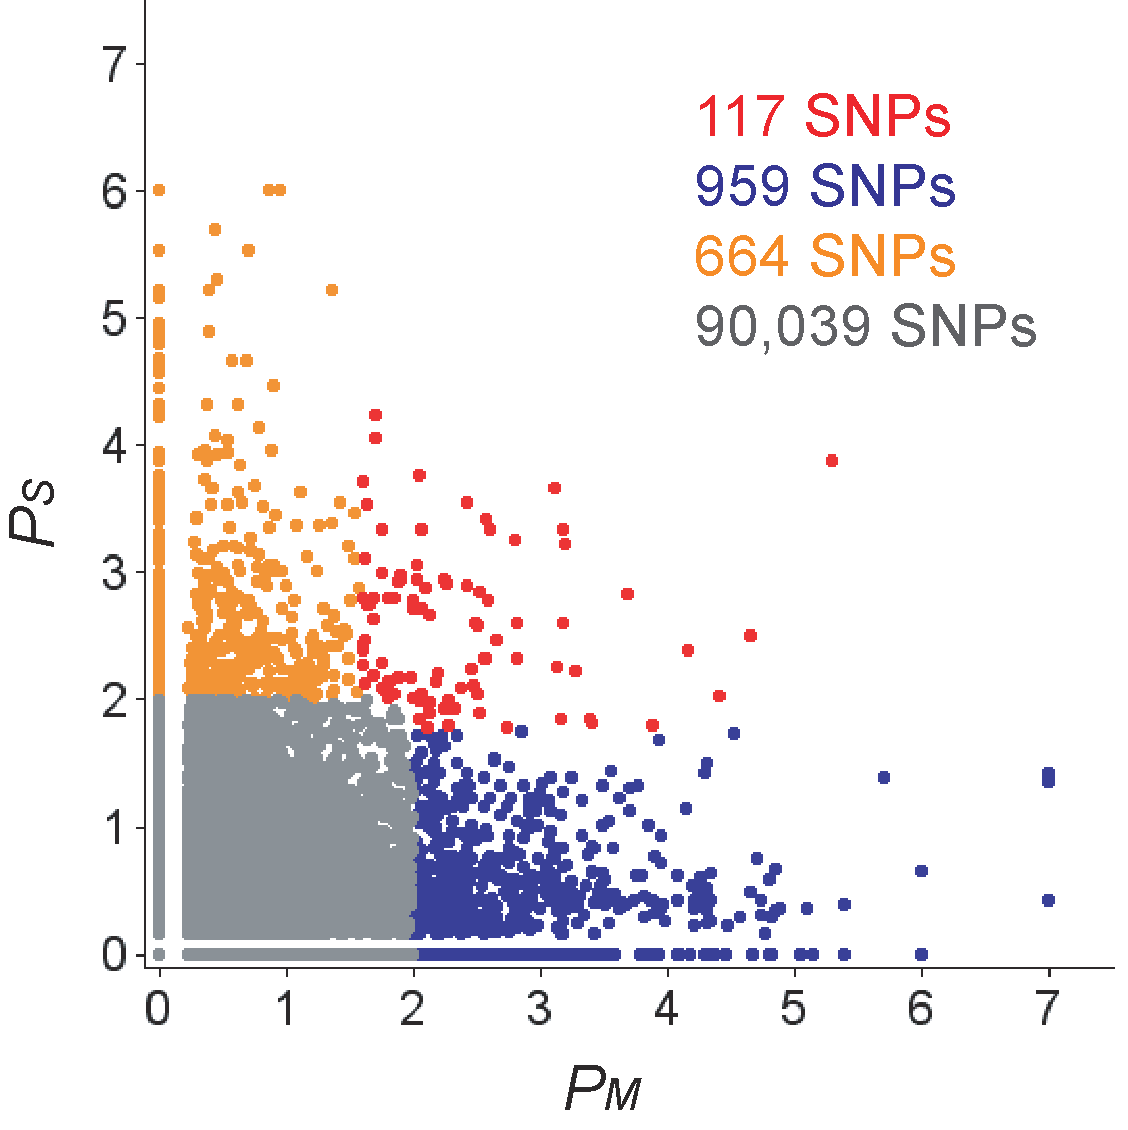
\includegraphics[width=0.4\textwidth]{fst.pdf}
  \caption{Scatter plot of $-\log_10 empirical P$-values of $F_{ST}$ values in Mexico ($P_M$ on $x$-axes) and South America ($P_S$ on $y$-axes).   Red, blue, orange and gray dots represents SNPs showing significance in both Mexico and South America, only in Mexico, or only in South America, respectively.  The number of SNPs in each category is shown in the same color of dots.} 
\end{SCfigure}


blah blah F$_ST$ \ref{fig:fst}.

%%%%%%%%%%%%%%%%%%%%%%%%%%%%%%%%%%%%%%%%%%%%%%%%%%%%%%%%%%%%%%%%%%%%%%
%SPECIFIC OBJECTIVES
%%%%%%%%%%%%%%%%%%%%%%%%%%%%%%%%%%%%%%%%%%%%%%%%%%%%%%%%%%%%%%%%%%%%%%
\section*{Specific Objectives}

%%%%%%%%%%%%%%%%%%%%%%%%%%%%%%%%%%%%%%%%%%%%%%%%%%%%%%%%%%%%%%%%%%%%%%
%AIM 1
%%%%%%%%%%%%%%%%%%%%%%%%%%%%%%%%%%%%%%%%%%%%%%%%%%%%%%%%%%%%%%%%%%%%%%

\renewcommand{\thesection}{Aim \arabic{section}}
\section{Genetic architecture of highland traits}

\subsection*{Questions}
\begin{itemize}
\item What is the genetic architecture of highland adaptation?
\item How much of the genetic architecture is shared between Mexico and South America?
\item How much of the genetic architecture is shared between maize and teosinte?
\item Are highland QTL/loci widespread in highland climes?
\end{itemize}

\subsection{QTL mapping of highland adaptation traits}
%\begin{itemize}
%\item Phenotyping at 4 sites: 
%\item 960 F2:3 families; 40 checks
%\item population development (RS, SFG)
%\item genotyping and mapping (JRI, SFG)
%\item DNA extraction, genotypes (SFG)
%\item Sequence parents (JRI)
%\item Mapping (SFG)
%\end{itemize}

In order to identify the genomic regions controlling highland adaptation in maize, we will conduct QTL mapping studies of one Mexican and one South American population, each derived by crossing an inbred landrace adapted to lowland conditions with a landrace adapted to highland conditions \ref{tab:qtlpops}.  We make use of specially-inbred landrace lines created by John Doebley (U. Wisconsin) and Seth Murray (Texas A\&M), thus simplifying downstream mapping applications and allowing replication of alleles in the our functional studies (see \ref{sec:funchar}). 

\begin{table}
\begin{center}
\caption{Parental lines for QTL} \label{tab:qtlpops}
\begin{tabular}{llll}\\\toprule  
{\bf Population}	& {\bf Parent } &	{\bf Origin (masl)} & {\bf Status }\\ \midrule
 \rowcolor{gray!25}
Mexico	& Zapalote Chico		& Oaxaca	 (46)		&  F2 \\ 
 \rowcolor{gray!25}
	& 	Palomero de Jalisco	& 	Jalisco (2520)		& \\
S. America	& Araguito	& Venezuela (183)	&  F1 \\ 
	& Sal Prieta	 & Ecuador (2948) & \\ \bottomrule
\end{tabular}
\end{center}
\end{table} 

Because we plan to evaluate these populations in replicated trials over multiple years, we will self-pollinate the F2 plants to create 500 F2:3 families from each population.  DNA will be extracted from each ofhte F2 plants and used for genotypic analysis.   The parents of the population will be sequenced to 20-30X depth on two lanes of Illumina 150bp paired-end, providing genome-scale SNP data similar in scale (tens millions of markers) to our previous work in maize  \citep[HapMap.v2;][]{Chia2012a}.  F2 plants will be genotyped using genotyping-by-sequencing \citep[GBS;][]{Elshire2011} and run through the standard maize GBS pipeline \citep{Glaubitz2014} resulting in approximately ~1M SNPs and allowing simple imputation of full-genome sequence.  The genetic map will be created using standard methods \citep[e.g.][]{Broman2003a}. 

\begin{table}
\rowcolors{2}{gray!25}{white}
\begin{center}
\caption{Common garden locations} \label{tab:locales}
\begin{tabular}{p{2cm}cccccc}\\\toprule  
{\bf Field Sites} & {\bf Lat/Lon } & {\bf Elevation\,(m) } &	{\bf Min/Mean/Max\,$^{\circ}\mathrm{C}$  } & {\bf Precip\,(mm) } \\ \toprule
Valle de Banderas, Nayarit	& 20.8,\,-105.2&	54		&	15.3/25.8/33.7	&	1184 \\
Irapuato, Guanajuato 	&	20.7,\,-101.3	&	1729.0	&	7.3/20.2/31.7	&	693 \\
Amealco, Quer\'etaro 	&	19.5,\,-99.1	&	2240.0 	&	2.3/15.6/27.0	&	626\\
Columbia, Missouri		& 	28.9,\,-92.2	&	266.1 	&	-17.8/36.0/40.5&	914\\
Ames, Iowa	& 	X	&	X 	&	X		&	X	 \\ \bottomrule
\end{tabular}
\end{center}
\end{table} 

The populations will be phenotyped at 3 field locations, including one lowland site (Valle de Banderas in Mexico), one highland site (Irapuato or Queretaro, Mexico), and one temperate site near Columbia, Missouri (\ref{tab:locales}).  In each location, the experiment will consist of two replications where the 500 entries and parental checks will be arranged in a randomized complete block design or an augmented alpha lattice design. The parental checks will be used to control for field variation.  We will collect a large number of phenotypes (\ref{tab:phenos}) using our in-house barcode-based data collection program. Germination at different planting depths and temperatures will be evaluated in controlled conditions in Ames, Iowa, and root chilling will be evaluated using a custom hydroponic system at the University of California, Davis (see letter of support from Dr. Arnold Bloom).    

%\begin{wraptable}{r}{8cm}
\begin{table}
\begin{center}
\rowcolors{2}{gray!25}{white}
\caption{Phenotypes measured}\label{phenos}
\begin{tabular}{llcc}\\\toprule  
{\bf Abbreviation} & {\bf Phenotype} & {\bf Lowland} & {\bf Highland } \\\midrule
MH & leaf sheath macrohairs & & \\
FT & flowering time & & \\
PH & plant height 			& & \\
BM & total plant biomass 	& & \\
EN & ear number			& & \\
FK & fifty kernel weight & & \\
TBN & tassel branch number & &\\
TL & tassel length & &\\
SM & total kernel mass & &\\
RC & root chilling response & &\\
GDP & germination depth & &\\
SC & stem anthocyanin content & &\\
GDP & germination depth & &\\
GDT & germination temperature & &\\\bottomrule
\end{tabular}
\end{center}it
\end{table} 

Raw data from each plot will be analyzed using mixed-models incorporating replications and environments.  Data will be analyzed across environments to determine whether location (elevation) affects the various phenotypes, as expected.  Each location will then be analyzed separately to derive least squares means to be used as the phenotypic data in QTL analyses.  QTL analysis will be conducted using standard, publicly available software (e.g. SAS; R/qtl \citealp{Broman2003a}).  Several iterations of QTL analysis will be conducted: on individual traits, individual traits adjusted for covariates such as flowering time, and multiple traits simultaneously.  The QTL profiles will be compared across populations (Mexican vs South American) and across field sites (elevations) to determine how elevation affects putatively adaptive traits.  We expect very different QTL profiles from the highland and lowland evaluation sites, and from the Mexican and South American populations.

%this needs something else. needs to talk about how we will answer questions above. that we will find how many QTL for each trait, that we expect this wil vary from fitness (yield) to color, thus informing us about the lability of these traits and how selection (or breeders) may act on them. also needs to mention fitness, no?  can we not use these pops to tell which traits are adaptive (i.e. genetically correlated to fitness/yield?)

\subsection{Admixture mapping in a teosinte hybrid zone}
%\begin{itemize}
%\item collection trip (MBH)
%\item 500 individuals from Ahuacatitlan in Mexico (MBH, RS)
%\item DNA extractions, genotyping (MBH)
%\item phenotyping (MBH, RS)
%\item mapping (MBH/GC)
%\end{itemize}


%\subsection{Phenotypes}
%\begin{itemize}
%\item macrohairs (SFG, RS, MBH)
%\item flowering time (SFG, RS, MBH)
%\item tassel morphology (SFG, RS, MBH)
%\item plant height every 2 weeks \& at flowering (SFG, RS, MBH)
%\item biomass (SFG, RS, MBH)
%\item \# ears (mz), 50k weight (mz/teo), total seed weight (mz) (SFG, RS, MBH)
%\item stem/plant color (SFG, RS, MBH)
%\item germination depth, temp in greenhouse (F2:3 only; MBH)
%\item roots (inquire with Bloom)
%\end{itemize}

\subsection{Global analysis of highland haplotypes}

\begin{itemize}
\item Occurrence of highland haplotypes/QTL/SNPs in global pops (MBH)
\item 500 worldwide accessions GBS (MBH)
\item Case study in Chihuahua (ACJ)
\item Berg's approach to show selection on traits in multiple highland popualtions
\end{itemize}


%%%%%%%%%%%%%%%%%%%%%%%%%%%%%%%%%%%%%%%%%%%%%%%%%%%%%%%%%%%%%%%%%%%%%%
%AIM 2
%%%%%%%%%%%%%%%%%%%%%%%%%%%%%%%%%%%%%%%%%%%%%%%%%%%%%%%%%%%%%%%%%%%%%%
\section{Adaptive introgression of highland alleles}

\subsection*{Questions}
\begin{itemize}
\item Are introgressed loci adaptive?
\item Does evidence of introgression and natural selection correspond to QTL?
\end{itemize}

\subsection{Population genetics of maize-teosinte introgression} \label{subsec: intropopgen}

GBS of 18 inds x 10 pops x 2 subspecies (mex \& maize) (JRI)
384 at 48 plex * \$60 = \$23040

Popgen on maize/mexicana introgression (JRI, GC)
Identification of fine-scaled introgressed regions.
Evidence of selection against introgression (recombination)
Evidence of selection for introgressed regions (sweep signals, deviation of genome-wide admixture signal)
Introgressed regions correlate with admix mapping signals? with QTL? Berg approach

\subsection{Population genetics of hybridization in teosinte} \label{subsec: admixpopgen}

make use of admixed pop sampled by matt
Berg approach of phenotypes mapped there for selection in parentals and hybrid

GBS Additional 5 admixed parv/mex populations (50 inds. each) (JRI)
also 4 new pops x (12 parv + 12 mex + 12 hybrids) = \$8160
Ahuacatitlan and 3 more
Introgression and adaptation in additional admix pops (JRI, GC)
Selection for/against regions in parv/mex/admix
Parallelism across pops in hybrid zone

%%%%%%%%%%%%%%%%%%%%%%%%%%%%%%%%%%%%%%%%%%%%%%%%%%%%%%%%%%%%%%%%%%%%%%
%AIM 3
%%%%%%%%%%%%%%%%%%%%%%%%%%%%%%%%%%%%%%%%%%%%%%%%%%%%%%%%%%%%%%%%%%%%%%
\section{Functional characterization of QTL} \label{sec:funchar}

\subsection{Questions}
\begin{itemize}
\item What do QTL/selected loci/introgressed loci do?
\end{itemize}

\subsection{Fine map pigmentation} \label{subsec:pigment}
\begin{itemize}
\item PT x T43 NIL population (RS)
\item GBS genotyping (MBH)
\end{itemize}

\subsection{Allelic series for QTL of interest} \label{subsec:series}
\begin{itemize}
\item 10 parents:
\begin{itemize}
\item 4 parents F2:3
\item mexicana TIL18
\item Palomero Toluqueño
\item 2 lowland landraces
\item 2 highland landraces
\end{itemize}
\item Cross into 3 parents for phenotyping
\begin{itemize}
\item B73 (SFG)
\item T43 (MBH)
\item CML457 (RS)
\end{itemize}
\end{itemize}

\subsection{RNAseq} \label{subsec:rnaseq}
\begin{itemize}
\item Time series analysis of plants in field (ACJ):
\item 15 Lines
\begin{itemize}
\item 4 F2:3 parents
\item 1 NIL chr4,
\item 1 each mex \& parv TIL
\item B73, CML457, T43, PT
\item highland/lowland landraces used in allelic series (MBH to inbreed)
\end{itemize}
\item 12 plants per line per environment (2 pools of 6)
\item 4 stages/tissues per plant
\item 2 environments (high/low fields)
\end{itemize}




\rowcolors{2}{gray!25}{white}
\begin{table}[H]
\begin{center}
\caption{Proposed timeline of activities and responsibilities}\label{timeline}
\begin{tabular}{lccccc}\\\toprule  
    \rowcolor{gray!50}
Year & 2015 & 2016 & 2017 & 2018 & 2019 \\\midrule
Objective \ref{subsec: series} Allelic series & 2015 & 2016 & 2017 & 2018 & 2019\\\midrule
Objective \ref{subsec: pigment} Fine mapping & -- & RS, AC & AC,JRI & AC,JRI & -- \\\midrule
Objective \ref{subsec: rnaseq} RNA-seq & 2015 & 2016 & 2017 & 2018 & 2019\\\midrule
Objective \ref{subsec: intropopgen} Maize/mexicana introgression & 2015 & 2016 & 2017 & 2018 & 2019 \\\midrule
Objective \ref{subsec: X} Admix mapping & 2015 & 2016 & 2017 & 2018 & 2019 \\\midrule
Objective \ref{subsec: X} QTL mapping & 2015 & 2016 & 2017 & 2018 & 2019 \\\midrule
Objective \ref{subsec: X} Highland haplotypes & 2015 & 2016 & 2017 & 2018 & 2019 \\\midrule
Objective \ref{subsec: admixpopgen} Admixture population genetics & 2015 & 2016 & 2017 & 2018 & 2019\\ \bottomrule
\end{tabular}
\end{center}
\end{table} 


\required{Broader Impacts}
% As in the project summary, broader impacts must be called out separately 
% in the project description.  You may be able to give more specific
% examples, or discuss how you've previously achieved these impacts.
% It should be similar, but not identical, to the Broader Impacts statement
% in the project summary

%Also mention online presence?  twitter, online dissemination, etc.? slideshare, figshare, preprints, Haldane's sieve?

\subsection*{Exchange Program} 

We propose an international student exchange program between the PIs in the U.S. and Senior Personnel at LANGEBIO in Mexico. Over the course of the grant, we propose to fund 10 graduate or undergraduate students for 3-month research internships in one of the collaborating laboratories. Students involved will participate in research projects directly relating to the research focus of the grant, including developing mapping populations, mapping traits, population genetic analysis, or analysis of next-generation data. The expectation is that such research will often lead to co-authorship on publications. Students will be asked to give two presentations, one to the host lab upon arrival, talking about the lab/university they came from and research there, and another to their host lab detailing their work over the 3-month period.  Each of the PIs will participate, sending students to Mexico and/or accepting students from Mexico for internships. PI Ross-Ibarra will manage the program, as he is fluent in Spanish and has past experience with a similar exchange program (NSF 0922703). Over the last four years, his lab has hosted 6 Mexican students who have worked on various computational aspects of centromere evolution. Two of those students have earned authorship on a paper to be submitted later this year and one has gone on to a PhD program in the U.S.

Our goal is to involve students directly in research while at the same time fostering intercultural exchange and promoting future international research opportunities. It is particularly appropriate for the study of maize, a crop with significant cultural and economic impact in both Mexico and the U.S. Participating Mexican students will learn new analytical methods -- especially computational management of large datasets -- that can be introduced to their respective laboratories and peers. American exchange students will similarly benefit from experience with large field experiments and efforts to functionally characterize individual loci.  The hope is that Mexican undergraduate students involved may be recruited to graduate programs in the U.S., ideally to work in the lab of one of the PIs, and that American undergraduate students will be exposed to international opportunities for research, graduate education, and collaboration.

\subsection*{Phenotyping workshop} %SFG, JRI

The USDA-ARS group in Columbia has developed a streamlined phenotypic data collection system utilizing a handheld barcode device, barcoded plant tags, and barcoded phenotyping tools in order to maximize efficiency.  We will host a phenotyping workshop in Columbia during each year of the grant.  Through this workshop, Dr. Flint-Garcia’s state-of-the-art system will be transferred to other research institutions to aid in large-scale data collection. The phenotyping workshop will include topics on Experimental Design, setting up the FieldBook database, and Data Collection.  Experimental design topics include understanding where variation comes from, how to control for environmental/field variability and experimental error; heritability and repeatability.  The need for consistent data collection and high-throughput will be emphasized.  FieldBook database setup topics include setting up Palm handheld users, locations, traits, projects, assigning plots to projects, assigning traits and measurements to projects,  generating barcoded plant tags, and loading the program and trait groups to the Palm to prepare for data collection.  Topics to be covered in Data Collection include data collection for specific traits related to local adaptation of interest to our group, synchronizing data from the palm with the desktop/laptop database, managing data conflicts between the palm and the database, running reports, and exporting data.  This proposal will provide travel support for instructors.  The workshop will be free but participants will be expected to purchase their own Palm handheld and pay for their own travel.  The workshop will be held each year in late summer so that the participants can gain hands-on experience in data collection in the corn field.

\subsection*{Software} %JRI and GC
\begin{itemize}
\item R code for novel analysis for admixed populations
\item Software \& pipelines on github 
\end{itemize}

%needs tweaking/cutting, currently verbatim from Coop's last grant.

A good understanding of population and quantitative genetics is key to a student’s understanding of genetics and evolution, but these subjects are often conceptually quite difficult. An understanding of genetic variation and its phenotypic effects is also an increasingly important part of being an informed citizen, due to the rise of personal genomics and genomic medicine \citep[e.g.][]{redfield2012}. The large amount of population genetic and association data being generated offers a superb chance to motivate these subjects using real – and pertinent - data. 
We will develop undergraduate teaching modules in population and quantitative genetics using publicly available human data. These modules will be tested and integrated into the large undergraduate teaching courses at UC Davis. We have already begun to develop and distribute some of these resources, e.g. genome-scale demonstrations of Hardy Weinberg Equilibrium (HWE) using the human HapMap data, see Figure 4. Such demonstrations underscore the usefulness of basic population genetics in describing real world patterns, and begin to expose students to the wealth of genomics data being collected. They also offer the chance to more easily teach more complex population genetics concepts. For example, in a mixed population sample the heterozygosity is reduced below the HWE expectation by a factor (1-FST); this can easily be seen and explained for a combined sample of Europeans and Africans (right-side of Figure 4)
Other examples will include: using height association data to demonstrate quantitative genetics models; and explaining concepts of genetic and genealogical ancestry using genomic identity by descent. We will also develop software to examine signals of selection around human adaptations, to allow students to examine the patterns of diversity around these loci in the common visual framework. These modules will be prepared in the open source statistical program R, to ensure that they are easily used, modified, and distributed, and to expose students to programming in biology. The modules will be designed so that they can be tailored for use at a variety of levels from teaching basic concepts to large undergraduate classes, to providing the raw data for programming exercises for upper division courses.

The modules will be publicly distributed (see Data Management Plan), and advertised via evoldir and other venues. We will be develop and archive the modules on github.com in a fully open manner. The use of github will allow others to modify and extend the modules and to share and track these modifications. We will regularly deposit updated versions of the modules into figshare and data dryad in order to ensure that a permanent resource is maintained. 

\subsection*{Germplasm resources} %MBH, SFG and RS

%need emphasis on germplasm we will create (mapping pops etc.) that will be in germplasm banks

The highland environment remains an important niche for global maize production, in terms of acreage and farmer involvement, if not overall yield. The highland environment presents a number of important abiotic challenges beyond high elevation per se, including periods of drought and cold, and highland adapted material has great potential to provide an important source of stress tolerance; the rapid development and inherent earliness of highland material, for example, may have general application in marginal environments. 

In Mexico, the highland niche represents a key target market for an emerging private sector of small breeding companies, established following deregulation in 1990s. While highland adapted hybrids are available, these are largely derived from lowland sub-tropical material with little or no contribution of the highland landraces. This project will move this important germplasm a step closer to breeding programs, and in doing so strengthen ties between the broader academic community (represented here by both US and Mexican institutions) and the Mexican private sector (letter of support UNISEM).

This project will also build further the collaboration between US institutions and LANGEBIO, with a number of Mexican graduate students being directly involved. While Mexican plant science retains a traditionally strength in biochemistry and molecular biology, genetics has been less well represented in recent years. As a consequence, while there is ready access to genomics technologies, the human resources to make the most of the opportunities they present may be lacking. This project provides an excellent opportunity for capacity building in a Mexican institution, with the expectation of a lasting impact through future collaboration.

\required{Results From Prior NSF Support}
% 5 pages or fewer of the 15 pages for entire description document.
% include results from NSF grants received in the past 5 years.
% If supported by more than one grant, choose the most relevant one.

% For each grant, include: 
%	(a) NSF award number, amount, dates of support 
%	(b) The title of this project
%	(c) Publications resulting from this research
%	(d) Summary of the results of the completed work
%	(e) A brief description of data samples available and other research products not described 	      elsewhere
%	(f) For renewed support, a description of the relationship between the completed and 			      proposed work

% Due to space limitations, it is often advisable to use citations rather
% than putting the titles of the publications in the body 
% of this section

\subsubsection*{Ross-Ibarra, Flint-Garcia: \#1238014: Biology of Rare Alleles in Maize and Its Wild Relatives}
\$13,311,185 (\$2,368,767 to Ross-Ibarra and \$1,206,211 to Flint-Garcia), 05/15/13-04/30/18. PI Edward Buckler, co-PIs J. Doebley, J. Holland, S. Flint-Garcia, Q. Sun, P. Bradbury, S. Mitchell, J. Ross-Ibarra
\par\noindent{\bf Intellectual merit}} In the first year we have developed accurate imputation approaches, found evidence for the importance of deleterious variants and non-genic polymorphisms in heterosis and GWAS, documented differences in recombination among the parents of the NAM population, and found population genetic evidence suggesting the importance of demography and purifying selection across the genome.   The grant has produced 18 total publications in its first year (only publications involving PIs Flint-Garcia and Ross-Ibarra are shown below). 
\par\noindent{\bf Broader impacts}  In the first year this project has included 10 postdoctoral and 12 graduate trainees. The GBS workshop and traveling maize exhibit continue to be popular and successful. A new version of the teacher-friendly guide to the evolution of maize has been revised and published online. 
\par\noindent{\bf Publications} \citet{peiffer2013genetic, Romay2013, wills2013many, Mezmouk2014, Peiffer2014, sood2014mining}

\subsubsection*{Ross-Ibarra: \#0922703: Functional Genomics of Maize Centromeres}
\$5,008,031 (\$754,409 to Ross-Ibarra). 09/01/09-08/31/14. PI Kelly Dawe, co-PIs J. Birchler, J. Jiang, G. Presting, J. Birchler, J. Ross-Ibarra
\par\noindent{\bf Intellectual merit} Centromeres are regions of the genome that organize and regulate chromosome movement, yet the biology of centromeres remains poorly understood. Co-PI Ross-Ibarra's group has focused in particular on the evolutionary genetics of centromeres. This work has demonstrated the remarkable evolutionary lability of centromere tandem repeats, but has shown that there is little evidence in maize for coevolution between centromere sequence and kinetochore proteins. Ongoing work from the Ross-Ibarra lab seeks to characterize kinetochore proteins, assess the phylogenetic evidence for longer-term coevolution, and understand patterns of centromere and genome size variation in natural populations. 
\par\noindent{\bf Broader impacts}  Co-PI Ross-Ibarra has established and currently runs an international student exchange program as part of this grant. Data and result of this project have been disseminated via publications and presentations as well as deposited in the maize genetics community database \url{www.maizegdb.org}. Former trainees on the grant include Dr. Matthew Hufford (Co-PI on the current grant). 
\par\noindent{\bf Publications} \citet{Shi2010a, Chia2012a, Fang2012a, Hufford2012, Hufford2012b, Hufford2013, Melters2013a, Kanizay2013, Pyhajarvi2013}

\subsubsection*{Coop: \#1262645: Collaborative Research: ABI Innovation: Visualization And Statistics For Spatial Population Genomic Analysis. }
\$314,260, with an effective date of 05/01/13. Award Duration: 36 months.
\par\noindent{\bf Intellectual merit} We are developing a set of spatial statistics methods based on Gaussian random fields for the analysis of geographic population genomics data. The first method based on this approach has just been published, allowing a sound statistical framework to distinguish the effects of geographic and ecological distance on genetic isolation. 
\par\noindent{\bf Broader impacts}  The R package of the software has been released online, and has already been used by many molecular ecologists. 
\par\noindent{\bf Publications} \citet{bradburd2013}

\subsubsection*{Flint-Garcia: \#0820619: Genetic Architecture of Maize and Teosinte}
\$ 9,823,000. 3/1/2009-2/28/2013. PI Edward Buckler, co-PIs J. Doebley, T. Fulton, S. Flint-Garcia, J. Holland, S. Kresovich, M. McMullen, Qi Sun. 
\par\noindent{\bf Intellectual merit}  This project extends over more than a decade, and has pioneered the characterization of population genetic and evolutionary parameters of maize diversity, developed resources to connect this genetic diversity to phenotype through both association and joint linkage-association mapping, conducted fine scale analysis of domestication and agronomic QTL, and recently expanded to whole-genome analysis of diversity, evolution, and phenotype. Overall, the maize diversity project has developed a wide range of approaches and broadened understanding of the maize genome, evolution and adaptation, genetic mapping, and the agricultural improvement of maize. The project successfully released and analyzed the maize Nested Association Mapping (NAM) population, collaborated on making first and second generation haplotype maps for maize, resolved domestication traits, developed a range of novel statistical approaches for association mapping, and dissected complex traits such as flowering time, kernel composition, disease resistance, height, and inflorescence and leaf morphology. 
\par\noindent{\bf Broader impacts} The outreach program included a traveling science museum exhibit on maize diversity, evolution and genetics (seen by at least 300,000 people at five venues to date, including the famous Corn Palace in South Dakota), online Teacher Friendly Guide to the Evolution of Maize, seven Genotyping-By-Sequencing (GBS) workshops (held at primarily at Cornell but has also been held in Kenya), and training of postdocs, graduate students and undergraduates, the vast majority of which have continued in scientific careers.  Former trainees on this grant include Dr. Flint-Garcia  and Dr. Ross-Ibarra  (PIs of the current grant), only their publications are shown below.
\par\noindent{\bf Publications} \citet{Buckler2009, Flint-Garcia2009, Flint-Garcia2009a, Flint-Garcia2009b, Gore2009, McMullen2009, Ross-Ibarra2009a, Bottoms2010, Dubois2010, Zhang2010a, vanheerwaarden2010a, vanheerwaarden2010b, Brown2011b, Morrell2011a, Studer2011b, vanheerwaarden2011a, Tian2011, Chia2012a, Cook2012a, Fang2012a, Hufford2012b, Hung2012, Hung2012a, Romay2013}
